%%%%%%%%%%%%%%%%%%%%%%%%%%%%%%%%%%%%%%%%%%%%%%%%%%%%%%%%%%%%%%%%%%%%%%%%%%
%%%%%                         CHAPITRE 3                            %%%%%%
%%%%%%%%%%%%%%%%%%%%%%%%%%%%%%%%%%%%%%%%%%%%%%%%%%%%%%%%%%%%%%%%%%%%%%%%%%

\lhead[\fancyplain{}{\leftmark}]%Pour les pages paires \bfseries
      {\fancyplain{}{}} %Pour les pages impaires
\chead[\fancyplain{}{}]%
      {\fancyplain{}{}}
\rhead[\fancyplain{}{}]%Pour les pages paires 
      {\fancyplain{}{\rightmark}}%Pour les pages impaires \bfseries
\lfoot[\fancyplain{}{}]%
      {\fancyplain{}{}}
\cfoot[\fancyplain{}{\thepage}]%\bfseries
      {\fancyplain{}{\thepage}} %\bfseries
\rfoot[\fancyplain{}{}]%
     {\fancyplain{}{\scriptsize}}


%%%%%%%%%%%%%%%%%%%%%%%%%%%%%%%%%%%%%%%%%%%%%%%%%%%%%%%%%%%%%%%%%%%%%%%%%%
%%%%%                      Start part here                          %%%%%%
%%%%%%%%%%%%%%%%%%%%%%%%%%%%%%%%%%%%%%%%%%%%%%%%%%%%%%%%%%%%%%%%%%%%%%%%%%

\chapter{Transmission de l'expertise humaine dans un jeu de données d'apprentissage}
\label{ch:dataset}

%============================================================================== Résumé du chapitre

\begin{center}
\rule{0.7\linewidth}{.5pt}
\begin{minipage}{0.7\linewidth}
\smallskip

\textit{
	L'identification d'un modèle à partir de résultats expérimentaux nécessite de disposer d'essais représentatifs pour le modèle.
	Dans ce chapitre, nous discuterons des méthodes de construction d'un tel jeu de données, dans le but de l'utilisation pour identifier un modèle par apprentissage statistique.
	En particulier, nous présenterons notre utilisation d'un plan d'expérience de criblage.
	De plus, l'annotation d'un jeu de données est une étape clé de l'apprentissage statique ; l'expert humain transfert sa connaissance au modèle.
	Nous présenterons la méthode d'évaluation de la qualité de pièces en plastiques que nous avons utilisée.
	Enfin, nous discuterons de la possibilité d'enrichir le jeu de données au fur et à mesure de la créations de nouveaux échantillons.
}

%\smallskip
\end{minipage}
\smallskip
\rule{0.7\linewidth}{.5pt}
\end{center}

\minitoc
\newpage

% \begin{raggedright}
\section{Construction d'un jeu de données représentatif} \label{sec:dataset_construction}
% \end{raggedright}
Tout système d'apprentissage statistique nécessite un jeu de données représentatif du modèle à construire.
Ces travaux nous ont permis d'évaluer différentes méthodes de construction du jeu de données d'apprentissage, vis à vis des contraintes industrielles.
Le Tableau \ref{tab:dataset} présente les méthodes que nous avons étudiées.

\begin{table}[h]
    \arrayrulecolor{black}
    \hspace*{-8mm}
    \begin{tabular}{|l|l|l|}
        \arrayrulecolor{black}
        \hline
        Méthode           & Avantage                                           & Inconvénient                                        \\ \hline
        \hline
        Plan d’expérience & Exploration de la plage de réglages  & Difficile à intégrer dans la démarche de production \\ \hline
        En ligne          & Pendant la phase de réglage du procédé & L’exploration dépend de la variabilité du procédé    \\ \hline
        Hors ligne        & Pendant la phase de réglage du procédé & Nécessite une traçabilité et un stockage rigoureux \\ \hline
    \end{tabular}
    \caption{Méthodes de construction du jeu de données d'apprentissage.}
    \label{tab:dataset}
\end{table}

\subsection{Exploration du procédé par plan d'expériences} \label{subsec:doe}
Pour construire un jeu de données représentatif du procédé d'injection-moulage et de la pièce en présence, il est nécessaire de parcourir la plus grande variété possible de réglages machine.

% \subsection{Optimisation par plan d'expériences} \label{subsec:doe}
Les plans d'expériences sont intéressants pour sélectionner les essais à réaliser pour modéliser un phénomène.
Il s'agit de méthodes qui permettent d'ordonner la réalisation d'essais expérimentaux et de spécifier les modifications à réaliser sur les variables.
L'objectif est de limiter le nombre d'essais à réaliser.
Il est également possible d'associer la complexité (ou le degré polynomial) du modèle, avec le nombre d'essais pouvant être réalisé.
Un petit nombre d'essais permettra de construire un modèle linéaire, tandis qu'un plus grand nombre d'essais pourrait permettre de réaliser un modèle quadratique.
En 1935, \citeauthor{fisher_design_1974} \cite{fisher_design_1974} propose un ouvrage de référence sur le sujet de la construction et de l'analyse des plans d'expériences.
Nous ne discuterons pas des critères d'optimalité des plans que nous présentons. Nous invitons le lecteur à se référer à cet ouvrage pour étudier cette notion importante pour la construction de plans utilisables.
La Figure \ref{fig:doe} représente l'espace de la valeur de trois variables comme un cube.
Les valeurs des trois niveaux des variables, obtenues pour différents plans d'expériences, sont représentées par les cercles.

\paragraph{Plan factoriel}\mbox{\label{parag:doe_factorial}} \\
Le \textit{plan factoriel} propose une recherche exhaustive de l'effet de la variation de chacune des variables.
Lorsque la variation des variables est réalisée sur deux niveaux distincts, il permet de construire un modèle linéaire.
Il permet également de rendre compte des interactions entre les variables.
Lorsque la variation des variables est réalisée sur trois niveaux distincts, il permet de construire un modèle quadratique.
Des modèles d'ordre supérieur peuvent être réalisés mais l'augmentation du $k$ nombre d'essais à réaliser suit alors une loi factorielle $2^k$.

\begin{figure}[t]
	\tikzset{
		vertex/.style={
			circle, minimum size=20pt, inner sep=0pt, fill=gray},
		axial/.style={
			circle, minimum size=20pt, inner sep=0pt, fill=gray!20},
		edge/.style={draw,thick,-,black},
		rotu/.style={midway},
		sinal/.style={draw, circle, inner sep=0pt, thin},
		empty/.style={circle, minimum size=20pt, inner sep=0pt, fill=white},
	}
	\def\dist{0.4}
	\def\ax{2}
	\centering
	\begin{subfigure}[b]{0.30\textwidth}
		\centering
		\resizebox{\linewidth}{!}{
			%\begin{adjustbox}{width=0.80\textwidth}
			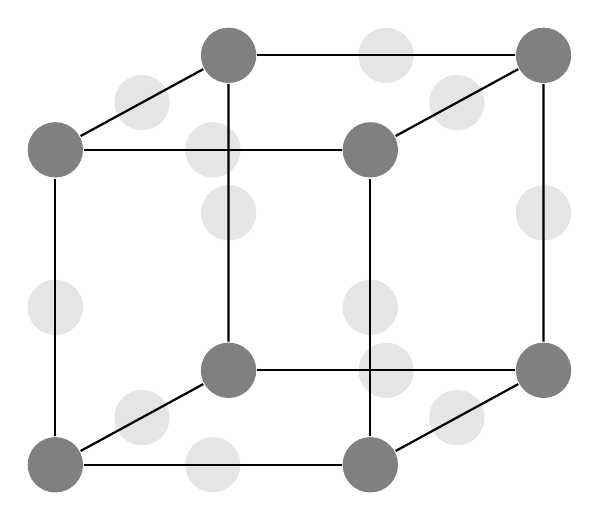
\begin{tikzpicture}[
			scale=2, ->, thick, z={(0.55,0.3)}, node distance=0.65cm, baseline]
			\node[vertex] (v0) at (-1,-1,-1) {};
			\node[vertex] (v1) at (-1,1,-1) {};
			\node[vertex] (v2) at (1,-1,-1) {};
			\node[vertex] (v3) at (1,1,-1) {};
			\node[vertex] (v4) at (-1,-1,1) {};
			\node[vertex] (v5) at (-1,1,1) {};
			\node[vertex] (v6) at (1,-1,1) {};
			\node[vertex] (v7) at (1,1,1) {};
			\node[axial] (c0) at (1,0,-1) {};
			\node[axial] (c1) at (1,0,1) {};
			\node[axial] (c2) at (-1,0,-1) {};
			\node[axial] (c3) at (-1,0,1) {};
			\node[axial] (c4) at (0,1,-1) {};
			\node[axial] (c5) at (0,1,1) {};
			\node[axial] (c6) at (0,-1,-1) {};
			\node[axial] (c7) at (0,-1,1) {};
			\node[axial] (c8) at (-1,-1,0) {};
			\node[axial] (c9) at (-1,1,0) {};
			\node[axial] (c10) at (1,-1,0) {};
			\node[axial] (c11) at (1,1,0) {};
			\draw[edge] (v0) -- (v1) -- (v3) -- (v2) -- (v0);
			\draw[edge] (v0) -- (v4) -- (v5) -- (v1);
			\draw[edge] (v2) -- (v6) -- (v7) -- (v3);
			\draw[edge] (v4) -- (v6);
			\draw[edge] (v5) -- (v7);
			\end{tikzpicture}
		}
		\newline
		\newline
		%\end{adjustbox}
		\caption{Plan factoriel.}
		\label{fig:doe_factorial}
	\end{subfigure}
	\begin{subfigure}[b]{0.32\textwidth}
		\centering
		\resizebox{\linewidth}{!}{
			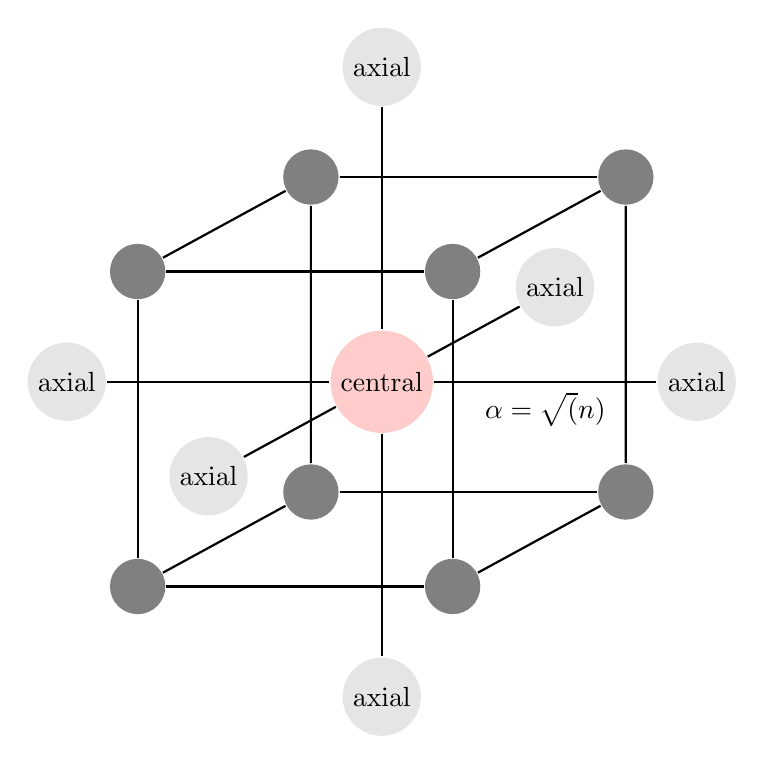
\begin{tikzpicture}[
			scale=2, ->, thick, z={(0.55,0.3)}, node distance=0.65cm]
			\node[vertex, fill=red!20] (c0) at (0,0,0) { \ central \ };
			\node[vertex] (v0) at (-1,-1,-1) {};
			\node[vertex] (v1) at (-1,1,-1) {};
			\node[vertex] (v2) at (1,-1,-1) {};
			\node[vertex] (v3) at (1,1,-1) {};
			\node[vertex] (v4) at (-1,-1,1) {};
			\node[vertex] (v5) at (-1,1,1) {};
			\node[vertex] (v6) at (1,-1,1) {};
			\node[vertex] (v7) at (1,1,1) {};
			\node[axial] (a1) at (-\ax,0,0) { \ axial \ };
			\node[axial] (a2) at (\ax,0,0) { \ axial \ };
			\node[axial] (a3) at (0,-\ax,0) { \ axial \ };
			\node[axial] (a4) at (0,\ax,0) { \ axial \ };
			\node[axial] (a5) at (0,0,-\ax) { \ axial \ };
			\node[axial] (a6) at (0,0,\ax) { \ axial \ };
			\draw[edge] (v0) -- (v1) -- 
			(v3) -- (v2) -- (v0);
			\draw[edge] (v0) -- (v4) -- (v5) -- (v1);
			\draw[edge] (v2) -- (v6) -- (v7) -- (v3);
			\draw[edge] (v4) -- (v6); \draw[edge] (v5) -- (v7);
			\draw[edge] (a1) -- (c0) -- (a2) node[rotu, below=0.1] {$\alpha=\sqrt(n)$};
			\draw[edge] (a3) -- (c0) --(a4);
			\draw[edge] (a5) -- (c0) --(a6);
			\end{tikzpicture}
		}
		\caption{Plan composite centré.}
		\label{fig:doe_cc}
	\end{subfigure}
	\begin{subfigure}[b]{0.30\textwidth}
		\centering
		\resizebox{\linewidth}{!}{
			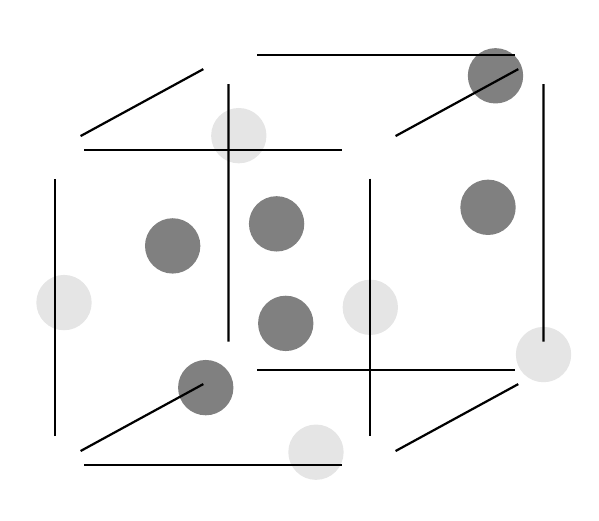
\begin{tikzpicture}[
			scale=2, ->, thick, z={(0.55,0.3)}, node distance=0.65cm]
			\node[empty] (v0) at (-1,-1,-1) {};
			\node[empty] (v1) at (-1,1,-1) {};
			\node[empty] (v2) at (1,-1,-1) {};
			\node[empty] (v3) at (1,1,-1) {};
			\node[empty] (v4) at (-1,-1,1) {};
			\node[empty] (v5) at (-1,1,1) {};
			\node[empty] (v6) at (1,-1,1) {};
			\node[empty] (v7) at (1,1,1) {};
			\node[vertex] (a1) at (-0.20, 0.20, 0.10) {};
			\node[vertex] (a2) at ( 0.75, 0.90, 0.90) {};
			\node[vertex] (a3) at (-0.10,-0.54,-0.90) {};
			\node[vertex] (a4) at (-0.75, 0.12,-0.10) {};
			\node[vertex] (a5) at ( 0.10,-0.30,-0.34) {};
			\node[vertex] (a6) at ( 0.95, 0.20, 0.45) {};
			\node[axial] (c0) at (1,0,-1) {};
			\node[axial] (c1) at (1,-0.9,1) {};
			\node[axial] (c2) at (-1,0,-0.9) {};
			\node[axial] (c3) at (0.6,-0.95,-0.9) {};
			\node[axial] (c4) at (0,1,-0.7) {};
			\draw[edge] (v0) -- (v1) -- (v3) -- (v2) -- (v0);
			\draw[edge] (v0) -- (v4) -- (v5) -- (v1);
			\draw[edge] (v2) -- (v6) -- (v7) -- (v3);
			\draw[edge] (v4) -- (v6);
			\draw[edge] (v5) -- (v7);
			\end{tikzpicture}
		}
		\newline
		\newline
		\caption{Plan hypercube latin.}
		\label{fig:doe_hls}
	\end{subfigure}
	\caption{Essais prévus pour des plans d'expériences à trois niveaux pour trois variables.}
	\label{fig:doe}
\end{figure}

\paragraph{Plan central-composite}\mbox{\label{parag:doe_cc}} \\
Le \textit{plan central-composite} (plan de \textit{Box-Wilson}) permet de construire des modèles d'ordre 3.
Il a été proposé dès 1950.
Il s'appuie sur un \textit{plan factoriel} à deux niveaux.
Ce modèle est complété en réalisant des essais pour les valeurs médianes des variables (appelés \textit{essais au centre}).
Enfin, on réalise des essais où chaque variable est ajustée indépendamment des autres (\textit{essais axiaux}).
Un coefficient $\alpha$ définit la valeur de la variation de la variable par rapport à l'essai au centre.
Pour un nombre $n$ de variables à étudier, on choisit généralement $\alpha = \sqrt{n}$.
D'autres méthodes de choix de $\alpha$ sont possibles et nous invitons le lecteur à consulter un ouvrage de référence sur la théorie des plans de surfaces de réponses tel que \citetitle{myers_response_1971} \cite{myers_response_1971}.
Le \textit{plan central-composite} réduit le nombre d'essais à réaliser en comparaison du \textit{plan factoriel}.
Le plan de \textit{Box-Behnken} propose de réduire le nombre d'essais en n'utilisant pas un plan factoriel comme plan de référence.
% Box-Behnken designs usually have fewer design points than central composite designs, thus, they are less expensive to run with the same number of factors. They can efficiently estimate the first- and second-order coefficients; however, they can't include runs from a factorial experiment. Box-Behnken designs always have 3 levels per factor, unlike central composite designs which can have up to 5. Also unlike central composite designs, Box-Behnken designs never include runs where all factors are at their extreme setting, such as all of the low settings.
Les plans de \citeauthor{plackett_design_1946} \cite{plackett_design_1946} proposent de réduire le nombre d'essais pour une étude à deux niveaux, dans le cas où le nombre d'essais est un multiple de 4 ($N=12, N=20, N=24 \dots$).
Ces plans sont idéaux pour réaliser une étude de nombreuses variables en peu d'essais et construire un modèle linéaire.

Nous utiliserons dans notre étude expérimentale un plan L12 de criblage afin de faire varier le procédé avec peu d'essais.
L'objectif sera de produire des pièces dont les caractéristiques sont les plus variées possibles.

\paragraph{Plan hypercube latin}\mbox{\label{parag:doe_lhs}} \\
L'objectif de ce plan est de couvrir la plage de valeurs des variables de manière quasi-aléatoire.
La méthode de construction de ce plan a été proposée par \citeauthor{mckay_comparison_1979} \cite{mckay_comparison_1979}. % Eglājs in 1977

Soit une grille à deux dimensions qui représente les valeurs de deux variables que l'on étudie.
On positionne sur cette grille des essais.
Cette grille est un \textit{carré latin} si elle ne contient qu'un unique essai par colonnes et par lignes.
Un \textit{hypercube latin} est la généralisation de ce principe pour une grille à $d$ dimensions.
Cette méthode garantit un positionnement quasi-aléatoire des essais dans l'espace de dimensions $d$.
À la différence des plans factoriels §\ref{parag:doe_factorial} ou composite centré §\ref{parag:doe_cc}, le nombre d'essais doit être connu pour construire le plan.
Cette méthode garantit que les essais soient réalisés sur l'ensemble de la variabilité du phénomène à modéliser ; à la différence d'un tirage aléatoire de la valeur des variables où il n'y a pas cette garantie.
Les plans d'hypercubes latins sont les plus utilisés dans la littérature de l'optimisation d'hyper-paramètres.

Il est également possible d'utiliser une séquence quasi-aléatoire pour réaliser le choix des essais.
La séquence de \citeauthor{sobol_distribution_1967} \cite{sobol_distribution_1967} est la plus utilisée dans la littérature.
Lorsque le nombre de variables est inférieur à $100$, elle permet une répartition plus intéressante que les hypercubes latins.
% A Sobol sequence is a low discrepancy quasi-random sequence. Sobol sequences were designed to cover the unit hypercube with lower discrepancy than completely random sampling (e.g. Random Search). Optunity supports Sobol sequences in up to 40 dimensions (e.g. 40 hyperparameters).
% The figures below show the differences between a Sobol sequence and sampling uniformly at random. These figures can be recreated using the code in bin/examples/python/sobol_vs_random.py.
% The mathematical details on Sobol sequences are available in the following papers: [SOBOL], [SOBOL2], [ANTONOV], [BRATLEY], [FOX].
% [SOBOL]   Ilya Sobol, USSR Computational Mathematics and Mathematical Physics, Volume 16, pages 236-242, 1977.
% [SOBOL2]  Ilya Sobol, Levitan, The Production of Points Uniformly Distributed in a Multidimensional Cube (in Russian), Preprint IPM Akad. Nauk SSSR, Number 40, Moscow 1976.
% [ANTONOV] Antonov, Saleev, USSR Computational Mathematics and Mathematical Physics, Volume 19, 1980, pages 252 - 256.
% [BRATLEY] Paul Bratley, Bennett Fox, Algorithm 659: Implementing Sobol’s Quasirandom Sequence Generator, ACM Transactions on Mathematical Software, Volume 14, Number 1, pages 88-100, 1988.
% [FOX] Bennett Fox, Algorithm 647: Implementation and Relative Efficiency of Quasirandom Sequence Generators, ACM Transactions on Mathematical Software, Volume 12, Number 4, pages 362-376, 1986.

% \paragraph{Plan de Taguchi}\mbox{\label{parag:doe_taguchi}} \\
% Bad and/or idocratic



\subsection{Sélection des paramètres de l'étude expérimentale} \label{subsec:l12_doe}
En amont de la réalisation des essais et du travail de modélisation, il est nécessaire de sélectionner les variables à étudier.
L'expertise des partenaires du projet FUI SAPRISTI a permis de retenir 11 variables pertinentes à prendre en compte dans la réalisation du plan de criblage.
Ces variables sont celles qui influencent le plus les caractéristiques des pièces plastiques.
Le Tableau \ref{tab:doe_choice} référence les variables de réglage du procédé que nous avons sélectionnées.
Les variables "critiques" ne sont pas étudiées dans le plan d'expériences.
En effet, leur bon réglage est nécessaire pour produire une pièce complète.
C'est pourquoi le réglage de ces paramètres est réalisé en amont du plan d'expérience, par un technicien-régleur expert.
Suite à la sélection des variables étudiés, un ordre de priorité est défini, d'après les connaissances des experts.

Le procédé d'injection-moulage est séquentiel, c'est pourquoi il est possible de régler certaines consignes sous la forme de séquences temporelles ; par exemple des paliers successifs de pression de maintien, en fonction de l'avancement du cycle d'injection.
En pratique, sur notre pièce simple, cette possibilité n'est pas réalisée.
Au contraire, en injection multi-buses séquentielle, le réglage des séquences temporelles est crucial pour obtenir une pièce de bonne qualité.
Le nombre de valeurs de réglages de ces paramètres séquentiels est très élevé, c'est pourquoi les plans d'expériences ne sont plus adaptés à leur étude exhaustive.
Un point de fonctionnement doit être initialement trouvé : c'est l'étape du réglage initial.
Elle est réalisée par le technicien régleur.
Par la suite, une exploration du procédé pourra être réalisée autour de ce point de fonctionnement.

\begin{table}[tbp]
    \centering
    \arrayrulecolor{black}\begin{tabular}{|l|l|l|l|l|l|l|}
        \arrayrulecolor{black}
        %\cline{1-1} \cline{3-6}
        \hhline{-~-----}
        Priorité &          & Variable de réglages          & Identifiant & Niveau -1 & Niveau 0   & Niveau 1   \\ \hhline{=:-:=:=:=:=:=:} %\hline
        1        & Critique & Vit. de rentrée des éjecters & /           & /         & optimale   & /          \\ \hline
        1        & Critique & Durée de maintien             & /           & 15 s      & 15 s       & 15 s       \\ \hline
        1        & Critique & Débit thermorégulateurs       & /           & /         & optimal    & /          \\ \hline
        1        & Critique & Course d'ouverture            & /           &           & optimale   & /          \\ \hline
        1        & Testée   & Température fourreau          & T-four      & 220°C     & 240°C      & 260°C      \\ \hline
        2        & Testée   & Temp. thermo-régulateurs      & T-therm     & 20°C      & 40°C       & 60°C       \\ \hline
        3        & Testée   & Pression de maintien          & P-main      & 100 hPa   & 200 hPa    & 300 hPa    \\ \hline
        4        & Testée   & Vit. d'ouverture outillage    & v-ouve      & 100 mm/s  & 110mm/s    & 120mm/s    \\ \hline
        5        & Testée   & Course d'injection            & C-com       & 80 cm$^3$ & 83 cm$^3$  & 86 cm$^3$     \\ \hline
        6        & Testée   & Vitesse d'injection           & v-inj    & 50 cm$^3$/s & 70 cm$^3$/s & 90 cm$^3$/s   \\ \hline
        7        & Testée   & Contre-Pression               & C-ouv       & 30 hPa    & 50 hPa     & 70 hPa     \\ \hline
        8        & Testée   & Délais de dosage              & t-reta      & 1 s       & 5 s        & 10 s       \\ \hline
        9        & Testée   & Vitesse de rotation de vis    & v-rot       & 50 tr/min & 100 tr/min & 150 tr/min \\ \hline
        10       & Testée   & Force de fermeture            & P-ferm      & 1000 kN   & 1500 kN    & 2000 kN    \\ \hline
        16       & Testée   & Course de dosage              & C-dos       & 90 cm$^3$ & 100 cm$^3$ & 110 cm$^3$    \\ \hline
    \end{tabular}
    \caption{Sélection des variables pour l'étude.}
    \label{tab:doe_choice}
\end{table}


% C'est l'intérêt des plans d'expériences.
L'analyse des résultats obtenus permet d'obtenir une modélisation de la réponse en fonction des valeurs des paramètres du procédé.
La réponse ici étudiée est la qualité de la pièce, c'est à dire ses caractéristiques.
% Les variables sont les réglages disponibles sur la machine.
Le modèle obtenu permet de mettre en évidence les paramètres les plus influents sur la qualité.
Il est alors possible de négliger les variables qui n'ont pas ou peu d'influence.
Nous n'avons cependant pas choisi d'exploiter cette information car nous cherchons à produire un moyen de mesure de la qualité adapté à différentes machines.
Le nombre d'essais réalisé dans le plan d'expériences est défini par le nombre de variables, le nombre de niveaux choisis et le choix de la construction du plan.
Dans le cas des plans factoriels, le nombre d'essais à réaliser augmente rapidement.
Dans le cadre d'une première série d'essais, il est intéressant de choisir un plan orthogonal à deux niveaux qui comporte peu d'essais.
Cela permettra d'étudier les interactions sous forme linéaire, afin de pouvoir affiner le modèle dans un plan suivant.

Nous avons conduit deux expérimentations par plans d'expériences sur des machines industrielles.
Dans un premier temps, un plan d'expérience de criblage \textit{L12} a été utilisé : 11 variables sur 2 niveaux \cite{plackett_design_1946}.
La Section \ref{subsec:doe} précédente discute des constructions possibles de plans d'expériences et de l'intérêt des plans de criblage.
Nous avons ajouté deux essais au centre pour étudier la répétabilité du procédé et deux essais de validation.
Notre plan est détaillés dans le Tableau \ref{tab:doe_screening}.
La réalisation pratique de ce plan d'expériences a demandé 4 journées de 8 heures.
Il a été choisi d'attendre la stabilisation du procédé avant de réaliser les mesures.
La production de 20 à 40 pièces est requise pour être certain de la stabilité.
Nous n'avons pas mesuré les 30 premières pièces produites lors du début de chaque expérience.
Du point de vue de l'organisation des essais, la contrainte principale est la capacité thermique du moule.
Aux vues de la masse d'acier en présence, la montée et la descente en température de l'outillage est très longue.
C'est pourquoi nous avons ordonné les essais pour réaliser une montée progressive de la température de l'outillage\footnote{En parallèle de ce travail de doctorat, \citeauthor{collomb_2018} a récemment proposé de réduire au maximum la capacité thermique de l'outillage et d'isoler les parois. Cela a permis de réduire le temps de cycle du moulage des composites \cite{collomb_2018}.
Il serait intéressant d'étudier cette démarche, par exemple est prenant en compte les déformations de l'outillage sous les contraintes pour l'alléger.}.

% Conditionnal formating table: https://tex.stackexchange.com/a/488568
\makeatletter
\newcommand*{\yncellcolor}{}
\def\yncellcolor\ignorespaces{\@ifnextchar{-}{\cellcolor{cyan!7}}{\@ifnextchar{1}{\cellcolor{orange!10}}{\@ifnextchar{0}{\cellcolor{gray!2}}{}}}}
\newcolumntype{m}{>{\yncellcolor}c}
\makeatother

% Please add the following required packages to your document preamble:
% \usepackage[table,xcdraw]{xcolor}
% If you use beamer only pass "xcolor=table" option, i.e. \documentclass[xcolor=table]{beamer}
\begin{table}[tbp]
    \centering
    \hspace*{-8mm}
    \arrayrulecolor{black}\begin{tabular}{m|m|m|m|m|m|m|m|m|m|m|m|}
        \arrayrulecolor{black}
        % \cline{2-12}
        \hhline{~-----------}
        & T-four & T-therm & P-main & v-ouve & C-com & v-inj & C-ouv & t-reta & v-rot & P-ferm & C-dos \\ \hhline{-:=:=:=:=:=:=:=:=:=:=:=} %\hline
        \multicolumn{1}{|r|}{Essai01} & -1     & -1      & -1     & -1     & -1    & -1    & -1    & -1     & -1    & -1     & -1    \\ \hline
        \multicolumn{1}{|r|}{Essai02} & -1     & -1      & -1     & -1     & -1    & 1     & 1     & 1      & 1     & 1      & 1     \\ \hline
        \multicolumn{1}{|r|}{Essai03} & -1     & -1      & 1      & 1      & 1     & -1    & -1    & -1     & 1     & 1      & 1     \\ \hline
        \multicolumn{1}{|r|}{Essai04} & -1     & 1       & -1     & 1      & 1     & -1    & 1     & 1      & -1    & -1     & 1     \\ \hline
        \multicolumn{1}{|r|}{Centré1} & 0      & 0       & 0      & 0      & 0     & 0     & 0     & 0      & 0     & 0      & 0     \\ \hline
        \multicolumn{1}{|r|}{Essai05} & -1     & 1       & 1      & -1     & 1     & 1     & -1    & 1      & -1    & 1      & -1    \\ \hline
        \multicolumn{1}{|r|}{Essai06} & -1     & 1       & 1      & 1      & -1    & 1     & 1     & -1     & 1     & -1     & -1    \\ \hline
        \multicolumn{1}{|r|}{Essai07} & 1      & -1      & 1      & 1      & -1    & -1    & 1     & 1      & -1    & 1      & -1    \\ \hline
        \multicolumn{1}{|r|}{Essai08} & 1      & -1      & 1      & -1     & 1     & 1     & 1     & -1     & -1    & -1     & 1     \\ \hline
        \multicolumn{1}{|r|}{Centré2} & 0      & 0       & 0      & 0      & 0     & 0     & 0     & 0      & 0     & 0      & 0     \\ \hline
        \multicolumn{1}{|r|}{Essai09} & 1      & -1      & -1     & 1      & 1     & 1     & -1    & 1      & 1     & 1      & -1    \\ \hline
        \multicolumn{1}{|r|}{Essai10} & 1      & 1       & 1      & -1     & -1    & -1    & -1    & 1      & 1     & -1     & 1     \\ \hline
        \multicolumn{1}{|r|}{Essai11} & 1      & 1       & -1     & 1      & -1    & 1     & -1    & -1     & -1    & 1      & 1     \\ \hline
        \multicolumn{1}{|r|}{Essai12} & 1      & 1       & -1     & -1     & 1     & -1    & 1     & -1     & 1     & 1      & -1    \\ \hline
        \multicolumn{1}{|r|}{Centré3} & 0      & 0       & 0      & 0      & 0     & 0     & 0     & 0      & 0     & 0      & 0     \\ \hline
        \multicolumn{1}{|r|}{Test1}   & 1      & 1       & 1      & -1     & -1    & 1     & -1    & -1     & 1     & 1      & -1    \\ \hline
        \multicolumn{1}{|r|}{Test2}   & -1     & -1      & -1     & 1      & 1     & -1    & 1     & 1      & -1    & -1     & 1     \\ \hline
    \end{tabular}
    \caption{Plan de criblage \textit{L12} utilisé.}
    \label{tab:doe_screening}
\end{table}

\subsection{Apprentissage en ligne}
Pour maximiser son adoption, un système de mesure de la qualité ne doit pas modifier le moyen de production en place : il doit être non invasif.
Il doit s'intégrer au procédé et aux pratiques métiers. La réalisation de plans d'expériences, afin de modéliser le procédé, est difficile à intégrer dans la pratique industrielle.
Les plans d'expériences sont conçus pour limiter le nombre d'essais, mais malgré cela, il est admis que la seule utilisation du savoir-faire du technicien-régleur est plus avantageuse pour régler le procédé.
Sur les pièces simples que nous avons pu étudier dans le cadre de ce travail, le technicien régleur est capable de régler le procédé d'injection pour obtenir une pièce de qualité satisfaisante en une trentaine de minutes, soit 30 pièces produites pour un temps de cycle de production d'une minute par pièce.
Deux solutions sont possibles :
\begin{itemize}
    \item Utiliser la phase de réglage, pilotée par le technicien-régleur, afin de recueillir des données variées.
    \item Automatiser la phase de réglages machines.
\end{itemize}

\subsubsection{Exploration humaine en cycle de production}
Nous avons conduit deux expérimentations sur des machines industrielles, sans planification préalable des configurations de réglages de la machine.
Ces essais ont permis d'obtenir des retours sur la faisabilité et la fiabilité de notre dispositif de mesure de la qualité.
Afin d'explorer les plages de fonctionnement des réglages du procédé, nous recommandons d'acquérir les données en particulier pendant ces évènements :
\begin{itemize}
\item pendant la phase de réglage,
\item pendant les défaillances du procédé,
\item pendant que certains asservissements du procédé sont arrêtés et que le procédé dérive.
\end{itemize}
Ces recommandations permettent de maximiser la variance du jeu de données.
Nous notons que c'est pendant la phase de réglages que la variance des données est maximale.
En effet, le réglage de la machine est un processus itératif qui nécessite d'appliquer successivement plusieurs points de fonctionnement au procédé.
Les 20 pièces produites pendant le réglage possèdent des caractéristiques de qualité variées.

\subsubsection{Pilotage automatique du procédé pour la création d'un jeu de données}
Nous définissons le pilotage d'un procédé comme la sélection d'un point de fonctionnement initial (phase de réglage), son optimisation et sa régulation.
Le réglage est aujourd'hui réalisé par un opérateur humain.
Dans le cas où la phase de réglage est automatisée, il devient possible d'explorer le procédé, tout en optimisant les réglages, à l'aide des méthodes d'optimisation que nous présentons dans la Section \ref{sec:auto_ml}.
Les plans d'expériences §\ref{subsec:doe} sont particulièrement adaptés à l'acquisition de données sur l'ensemble de l'espace de fonctionnement d'un procédé.
Il est possible de compléter un plan d'expériences par de nouveaux essais, dans les plages de réglages qui possèdent les meilleurs performances.


\bigskip

\miniconclusion{Conclusion}{
	Pour identifier le modèle d'un phénomène à partir de mesures expérimentales, il est nécessaire de réaliser des mesures qui sont représentatives du phénomène.
	Dans le cas contraire, le modèle est partiel, voir biaisé.
	
	Les plans d'expériences permettent de produire des pièces dont la variabilité des caractéristiques est représentative de l'ensemble de la plage de fonctionnement d'un procédé de fabrication.
	
	Nous avons présenté le choix de la table L12 de criblage, ainsi que les paramètres qui seront modifiés dans le cadre de nos essais expérimentaux.
	
	Enfin, nous présentons la démarche d'apprentissage en ligne, c'est à dire que le jeu de données est construit au fur et à mesures de la production, sans planification initiale.
	À terme, le pilotage du procédé pourra permettre de réaliser une exploration automatique de la plage de fonctionnement du procédé.
}

\newpage

\section{Annotation humaine du jeu de données en contexte industriel}
C'est par l'annotation d'un jeu de données que l'expert humain transfert sa connaissance au système informatique.

Nous distinguons deux méthodes d'annotation humaine d'un jeu de données d'apprentissage :
\begin{itemize}
    \item l'annotation "hors ligne", qui est effectuée à posteriori de la production des données,
    \item l'annotation "en ligne", qui est effectuée pendant la production des données.
\end{itemize}
Dans le cadre de la pratique industrielle, on parlera d'annotation "en ligne" lorsqu'elle est réalisée au fur et à mesure de la production des pièces.
Dans ce cas, l'annotation est effectué directement depuis la ligne de production.
À contrario, l'annotation hors ligne peut être réalisée en dehors de la ligne de production.

Une des principales limites au déploiement de système par apprentissage est le coût de l'annotation.
En effet, le coût de l'annotation humaine est conséquent car il monopolise un expert du domaine.
En 2015, \citeauthor{bearman_what_2015} évalue les durées moyennes de différents types d'annotations \cite{bearman_what_2015}.
% https://hbilen.github.io/wsl-cvpr18.github.io/assets/wsod.pdf
% Berman et al., What’s the Point: Semantic Segmentation with Point Supervision, ECCV 16
Le Tableau \ref{tab:annotation} présente ces résultats.
Dans le cadre industriel, la durée d'annotation définit le coût économique du travail de l'expert qualité qui la réalise.
Ainsi, il n'est pas envisageable de réaliser une segmentation précise depuis une ligne de production.
Nous discuterons dans la suite de la faisabilité de l'annotation d'un jeu de données dans un contexte industriel.

\begin{table}[tb]
	\centering
	\arrayrulecolor{black}
	\begin{tabular}{|l|r|r|c|}
		\arrayrulecolor{black}
		\hline
		Méthode & Durée par classe & Qualité de localisation & Illustration de l'annotation\\
		\hline
		\hline
		Label de présence & 1,0 s & Aucune localisation & \includegraphics[width=3.5cm,keepaspectratio,valign=c,margin=1mm 1mm]{../Chap3/Figures/163-35_r.jpeg}
		\\
		\hline
		Label + point & 2,4 s & Localisation globale & \includegraphics[width=3.5cm,keepaspectratio,valign=c,margin=1mm 1mm]{../Chap3/Figures/163-35_r_point.jpeg} \\
		\hline
		Label + rectangle & 10 s & Localisation locale & \includegraphics[width=3.5cm,keepaspectratio,valign=c,margin=1mm 1mm]{../Chap3/Figures/163-35_r_box.jpeg} \\
		\hline
		Label + masque & 78 s & Segmentation précise & \includegraphics[width=3.5cm,keepaspectratio,valign=c,margin=1mm 1mm]{../Chap3/Figures/163-35_r_segm.jpeg} \\
		\hline
	\end{tabular}
	\caption{Durées d'annotations moyenne d'une image pour un humain.}
	\label{tab:annotation}
\end{table}

\subsection{Annotation hors ligne}
Nous proposons une méthode de notation de la qualité basée sur l'expertise humaine.
De précédents travaux sur l'évaluation visuelle de la qualité par de multiples experts ont montrés la difficulté d'accorder les avis d'experts humains \cite{baudet_visual_2011}.
\citeauthor{baudet_visual_2011} étudie l'évaluation de la qualité de 18 produits, par un panel de cinq contrôleurs humains.
Les résultats de l'évaluation de ce panel possédaient une variance maximale de 50\% sur l'ensemble des niveaux de qualité, .
Cette variance est très élevée ; elle n'est pas acceptable pour un moyen de mesure.
Cette étude montre qu'il est nécessaire de formaliser l'évaluation.
Il faut également former les contrôleurs humains pour harmoniser les évaluations.
% Une analyse R\&R aurait pu être effectuée pour mesurer la précision de notre méthode.
Afin d'évaluer la variabilité des évaluations humaines,  \citeauthor{baudet_maitrise_2012} \cite{baudet_maitrise_2012} propose une évolution de la méthode \textit{R\&R} (\textit{Repetability \& Reproductibility}) qui a été initialement proposée par le \citeauthor{automotiveindustryactiongroup_measurement_2010} pour évaluer la variabilité des moyens de mesure \cite{automotiveindustryactiongroup_measurement_2010}.
La variabilité peut avoir deux causes : un problème de répétabilité de la mesure ou un problème de reproductibilité.
Pour que le système de mesure soit conforme et puisse être utilisé, la pratique industrielle accepte généralement une variabilité inférieure à 30\%
Dans notre cas, nous chercherons à concevoir un système de contrôle qui réalisera moins de 10\% d'erreurs de classification.

\paragraph{Expérimentation de l'annotation hors ligne}\mbox{} \label{parag:offline_annotation} \\
Sur notre cas d'application "boîte noire", présenté dans le Chapitre \ref{ch:measure}, nous avons expérimenté une méthode de construction d'une métrique de la qualité des pièces.
L'échelle de notation est construite au fur et à mesure, par comparaison entre les niveaux de défauts des pièces.
Les pièces sont classées sur une grande table, par comparaison manuelle.
Afin d'obtenir une évaluation répétable et reproductible de la qualité, ce classement est réalisée par quatre experts humains qui débattent jusqu'à être d'accord.
Nous justifions cette démarche par la nécessité de limiter la dispersion inter-classes.
Si nous ne sommes pas capables de différencier deux pièces, alors ces pièces appartiennent à la même classe.
Nous n'avons pas réalisé d'analyse de répétabilité \textit{R\&R} du panel de quatre experts.
C'est une perspective intéressante pour des travaux complémentaires.

\begin{figure}[bt]
	\centering
	\begin{subfigure}[c]{0.70\textwidth}
		\includegraphics[width=1\textwidth,height=\textheight,keepaspectratio]{../Chap3/Figures/annotation_1.jpg}
	\end{subfigure}
	\begin{subfigure}[c]{0.29\textwidth}
		\centering
		\includegraphics[width=1\textwidth,height=\textheight,keepaspectratio]{../Chap3/Figures/annotation_2.jpg}
	\end{subfigure}
	\caption{Annotation hors-ligne par les experts humains.}
	\label{fig:annotation}
\end{figure}
Les photographies de la Figure \ref{fig:annotation} présentent la réalisation de l'annotation hors-ligne.
Les numéros sous les colonnes de pièces indiquent la valeur attribuée à chaque colonne sur l'échelle de qualité.
L'échelle a été construite de manière dynamique.
Elle va de 1 : le niveau de qualité le meilleur ; à 7 : les pièces qui possèdent les pires caractéristiques du point de vue de la qualité.

Il s'est avéré difficile pour les contrôleurs humains de donner une note qui prend en compte plusieurs types de défauts.
Les contrôleurs experts possèdent un a-priori de la notion de qualité qui s'appuie sur des types de défauts.
C'est pourquoi nous avons identifié trois défauts présents sur les : la retassure, le givrage et les brulures.
La démarche de notation par comparaison a été réalisé trois fois de suite, pour les trois types de défauts différents.
Une moyenne géométrique des notes combine les trois types de défauts et produit l'évaluation finale de la qualité de chaque pièce.

\noindent
Nous identifions trois limites à ce processus d'annotation humaine :
\begin{itemize}
\item La durée de 3 heures avec 3 experts pour évaluer 200 pièces, soit 60 pièces par heure. Cette cadence est équivalente au temps de cycle de production d'une pièce par heure.
\item La surface de travail nécessaire pour organiser les pièces et que les trois experts puissent les manipuler librement.
\item Les risques liés à la détérioration des pièces entre leur production et l'étape d'annotation.
\end{itemize}
C'est pourquoi, nous recommandons de réaliser l'annotation au plus près du procédé d'injection-moulage ; si possible dès la sortie des pièces du moule d'injection.

\subsection{Annotation en ligne de production}
Réaliser l'annotation en ligne de production permet d'éliminer deux risques d'erreurs critiques sur le jeu de données d'apprentissage :
\begin{itemize}
    \item la modification des pièces entre leur production et leur annotation
    \item l'erreur d'annotation à posteriori : l'expert peut ici observer la pièce
\end{itemize}

En contrepartie, la durée disponible pour l'annotation est très limitée. En plus de la durée de l'annotation, l'expert humain doit assister les opérations de manutention des pièces et les opérations connexes.
Nous estimons la disponibilité de l'expert humain à une trentaine de secondes pour un temps de cycle de procédé d'une minute.

Le Tableau \ref{tab:annotation} présente les durées moyenne de la tâche d'annotation.
Dans le cas d'une annotation au fil de la production de pièces, il n'est pas envisageable de réaliser une segmentation précise, à cause de sa durée élevée.
Nous obtenons de ces résultats l'intérêt de réaliser une annotation rapide, sans nécessairement chercher à localiser les défauts.
Indiquer la présence ou l'absence de défauts est rapide.
Ensuite, nous pouvons préciser le niveau de la qualité en proposant une échelle discrète simple, par exemple à cinq niveaux de qualité.
Afin de répondre à ce problème de vitesse d'annotation, une interface logicielle a été spécifiquement développée.
Nous discutons de cette interface dans le Chapitre \ref{ch:theeye}.

\subsection{Intégration de l'humain dans le système d'apprentissage}
L'expertise humaine est indispensable à la modélisation par apprentissage statistique.
L'humain doit transférer ses connaissances holistiques au logiciel informatique.
C'est pourquoi, il nous paraît indispensable d'intégrer l'humain au plus près du processus d'apprentissage.
Cela nécessite une interface adaptée.
Par ce biais, l'expert humain peut effectuer deux actions :
\begin{itemize}
    \item identifier la cause du défaut,
    \item alerter si le modèle statistique donne une information erronée.
\end{itemize}

Afin de motiver l'expert humain à transmettre ses connaissances au système informatique, la ludification du processus d'annotation peut aussi être un facteur important.
De nombreuses sociétés informatiques l'ont bien compris et nous annotons actuellement de manière naturelle et transparente des bases de données d'apprentissage : par le biais de notre navigation sur l'Internet ou des interactions avec notre smartphone, et de toutes les données recueillies par les capteurs connectés.
Le déploiement d'un système d'évaluation de la qualité dans les ateliers de production sera facilité par l'attrait de l'interaction avec l'interface d'annotation.

Nous avons développé une solution logicielle afin de résoudre ce problème.
Nous présenterons nos développements logiciels dans le Chapitre \ref{ch:theeye}.
Une interface sur navigateur web est accessible depuis tous les terminaux.
Tout au long de la production de nouvelles pièces, celles-ci s'affichent en temps réel et l'expert humain peut annoter la qualité.
L'annotation peut être réalisée depuis la ligne de production, ce qui permet le contrôle visuel direct des pièces.
L'annotation peut également être effectuée à distance : dans ce cas, l'expert humain se base sur l'image enregistré par le dispositif de mesure pour évaluer la qualité.
Dans le cas de pièces techniques à haute valeur ajoutée, la présence de l'expert sur la ligne est recommandée.
Il peut ainsi manipuler les pièces pour réaliser une annotation précise.

\subsection{Assistance à l'annotation humaine} \label{subsec:labelling_assistance}
% Dans certains cas, l'expertise humaine ne permet pas de différencier la qualité entre deux pièces.
La disponibilité de l'expert humain est limitée.
Il est possible de l'assister dans la tâche d'annotation.
Il est également possible de limiter le nombre d'annotations à réaliser aux cas les plus critiques.
Deux démarches peuvent être réalisées en parallèle : suggérer et détecter les pièces nouvelles, qui sont pertinentes à annoter.

\subsubsection{Suggestion d'annotations}
Dans certains cas, l'expertise humaine ne permet pas de différencier la qualité entre deux pièces.
Plusieurs limites humaines peuvent être la cause d'une telle situation :
\begin{itemize}
    \item L'expert ne peut pas mémoriser les caractéristiques de l'ensemble des pièces produites.
    \item L'expert humain ne peut pas comparer les pièces car les pièces ne lui sont plus accessibles.
    \item L'expert humain ne dispose pas d'assez de temps pour comparer les pièces.
\end{itemize}

Il est alors intéressant de suggérer à l'expert humain une annotation.
De plus, si cette suggestion est motivée par un argumentaire, elle sera d'autant plus crédible.
Il ne faut néanmoins pas influencer l'expert humain.
C'est pourquoi cette suggestion ne doit être effectuée que lorsque le niveau de confiance du modèle statistique est élevée.
Des les autres cas, il vaudra mieux écarter la pièce incertaine du jeu de données d'apprentissage.
Nous recommandons une certitude de classification supérieure à 90\% pour suggérer une annotation.

Pour suggérer la catégorie de la pièce, les méthodes de \textit{clustering} permettent d'identifier des paquets de pièces similaires.
Pour suggérer, il faut également justifier.
Il est nécessaire de transmettre à l'expert humain l'information.
C'est pourquoi, l'affichage sous forme d'un graphique des paquets de pièces similaires est utile.
Les algorithmes \textit{ACP} \ref{subsubsec:ACP}, \textit{t-SNE} \ref{subsubsec:tsne} ou \textit{UMAP} \ref{subsubsec:umap} permettent de projeter un espace de grandes dimensions dans un graphique à deux ou trois dimensions.
Nous détaillons leur application dans la Section \ref{subsec:unsupervised}.
Ce graphique peut être interprété par un humain.
Sur ce graphique, nous ajoutons l'affichage automatique de l'image de chaque pièce lors du survol des points.
Cela permet d'identifier les paquets de pièces similaires très rapidement, mais aussi les erreurs de classifications (humaine où du système automatique).


\subsubsection{Détection de nouveautés}
Dans le cas spécifique des productions industrielles sur des procédés stables, la majorité des pièces produites sera de bonne qualité.
C'est pourquoi, la tâche d'annotation de toute la production industrielle sera laborieuse pour l'expert humain et aura peu d'intérêt pour le modèle.
Aussi, la variabilité maximale sur les procédés industriels est produite lors de la phase de réglage du procédé.
Il est capital d'annoter les pièces issues de cette phase.
Par la suite, les pièces seront similaires et de bonne qualité.
De plus, différents points de fonctionnement du procédé peuvent amener à la production de pièces similaires, car le procédé d'injection moulage est non-bijectif, à cause de la multiplicité de ses paramètres réglables et de leurs réponses non-linéaires.
Il est ainsi nécessaire de mettre en évidence les pièces qui présentent de l'intérêt pour la base d'apprentissage : c'est à dire les pièces qui sont "nouvelles".
Des méthodes d'analyses de données sans supervision permettent de réaliser cette tâche.
Nous détaillons l'application de ces méthodes dans la Section \ref{subsec:unsupervised}.
Nous présentons ici les deux méthodes que nous avons implémentées, la mesure de distance de Mahalanobis et la machine à vecteurs de support à une classe.

\paragraph{Mesure de distance dans un espace réduit par l'Analyse en Composante Principale}\mbox{} \\
% https://scikit-learn.org/stable/auto_examples/plot_anomaly_comparison.html#sphx-glr-auto-examples-plot-anomaly-comparison-py
Il s'agit de réduire l'espace des données en projetant les valeurs dans un espace de dimensions réduite.
L'Analyse en Composantes Principales §\ref{subsubsec:ACP} réduit l'espace des données initial en combinant les relations linéaires existantes entre les composantes.
On choisit la dimension de l'espace de donnée réduit est choisi afin de limiter la perte d'informations à partir de l'espace initial.
Cette perte d'information est mesurée par l'écart de la variance exprimée.
Dans notre cas spécifique, la dimension des données d'entrés sont des images qui comportent près d'un million de pixels.
Nous projetons ces valeurs dans un espace de dimensions 100.
La perte de variance est alors inférieure à 0,01\%.

Dans cet espace de données réduit, il devient possible de mesurer la distance entre les points.
La distance euclidienne ne prend pas en compte les corrélations entre les variables, c'est pourquoi la distance de Mahalanobis \cite{mahalanobis_generalised_1936}, Équation \ref{eq:mahalanobis}  est couramment employée pour mesurer des distances entre paquets d'échantillons.
La distance de Mahalanobis entre un paquet de pièces de références et une pièce nouvelle est représenté par une ellipse.
% D'autres distances peuvent également être utilisées : Earth Mover, Cosinus, Jacquard.

\begin{equation} \label{eq:mahalanobis}
D_{Mahalanobis}(x, y)=\sqrt{(x - y)^{T} \Sigma^{-1}(x-y)}
\end{equation}

% TODO: Mahalanobis FIGURE
Pour obtenir un détecteur de nouveauté, il reste à définir un seuil à partir duquel la pièce est considérée comme mauvaise.
Ce seuil est soit imposé, soit défini de manière automatique.
Dans le cas d'un seuil automatique, on choisira un seuil égal à la distance de Mahalanobis de l'ensemble des pièces actuellement dans la base d'apprentissage ; ce sont les pièces existantes et nous cherchons à détecter les nouvelles.
La distance de toute pièce nouvelle dépassera alors ce seuil et la nouveauté sera détectée.
Cette démarche est employée avec succès dans les travaux de \citeauthor{lacombe_exploitation_2018a} sur le contrôle visuel automatique par système multi-éclairage, afin de détecter les pièces conformes et les pièces non-conformes \cite{lacombe_exploitation_2018a}.
% https://scikit-learn.org/stable/auto_examples/covariance/plot_mahalanobis_distances.html
% Rousseeuw, P.J., Van Driessen, K. “A fast algorithm for the minimum covariance determinant estimator” Technometrics 41(3), 212 (1999)

\paragraph{Machine à Vecteurs Supports à une classe}\mbox{} \\
À partir d'un classifieur machine à vecteurs de support §\ref{parag:svm}, \citeauthor{scholkopf_support_1999} proposent de chercher à classifier l'ensemble des données existantes dans une unique classe \cite{scholkopf_support_1999, scholkopf_estimating_2001}.
C'est la méthode \textit{One-Class SVM}.
À l'aide de noyau gaussien, cette méthode permet de prendre en compte des données aux propriétés plus complexes, que la matrice de covariance précédente de la distance de Malhanobis.
Le paramètre de marge $b$ correspond à la probabilité de classifier un nouvel échantillon, qui serait situé en dehors de l'hyperplan de marge maximal, comme nouveau.
% TODO: One-Class SVM: Figure de résumé de la démarche

%\subsubsection{Local Outlier Factor (LOF)}
% In anomaly detection, the local outlier factor (LOF) is an algorithm proposed by Markus M. Breunig, Hans-Peter Kriegel, Raymond T. Ng and Jörg Sander in 2000 for finding anomalous data points by measuring the local deviation of a given data point with respect to its neighbours.[1]
%
% LOF shares some concepts with DBSCAN and OPTICS such as the concepts of "core distance" and "reachability distance", which are used for local density estimation.[2]

%\subsection{Construction du jeu d'apprentissage en parallèle sur de multiples machines : Détection de similitudes}
% TODO: il est nécessaire de disposer d'un gros jeu de données par machines pour devenir robuste aux machines.
%Il est courant dans l'industrie de disposer de plusieurs lignes de production pour produire une même pièce.
%Nous n'évoquons pas dans ce travail le cas des moules à empreintes multiples, mais uniquement de multiples machines d'injection-moulage.
%Dans le cas où la construction du jeu de données d'apprentissage est effectuée sur de multiples machines, il est possible de centraliser un modèle de contrôle de la qualité.
%
%Nous obtenons un système similaire à la méthode faiblement supervisé d'apprentissage par curriculum, à la différence que l'expert humain est ici intégré dans le système.
%L'expert humain agit en temps que modèle de référence.

\paragraph{Détection de modifications sur le procédé}\mbox{} \label{subsec:labelling_detection} \\
Une approche complémentaire, pragmatique, à ce problème est de réaliser la détection de l'intervention du technicien humain sur les réglages du procédé.
En effet, lorsque le technicien modifie les réglages, il cherche nécessairement à optimiser la qualité des pièces produites.
Il suffit alors d'ajouter à la base de données d'apprentissage les pièces pour lesquelles une intervention humaine sur les réglages a eu lieu.
De manière pratique, le système d'apprentissage doit disposer d'une mémoire tampon où quelques dernières pièces produites sont conservées.
En cas d'intervention humaine sur les réglages du procédé, cette mémoire tampon est ajoutée à la base d'apprentissage.
Nous ajouterons également un certain nombre de pièces produites à la suite avec les nouveaux réglages.
Nous proposons d'ajouter un nombre de pièces qui correspond à la variabilité court-terme du procédé.
Dans le cas de l'injection des thermoplastiques, suite à un réglage, une dizaine de pièces permettent de stabiliser le procédé.
C'est pourquoi nous proposons d'enregistrer deux pièces précédant la modification des réglages, ainsi que les dix pièces suivant la modification.
Cette contrainte dimensionne la capacité de mémoire informatique du système d'apprentissage.
Dans le cas de douze pièces, la mémoire tampon sera de l'ordre de mille mégaoctets.

Nous n'avons pas pu évaluer notre proposition dans le cadre de ce travail, car cela nécessite l'enregistrement automatique de la valeur des réglages de la machine.
Cette intégration doit être réalisée en lien avec les constructeurs des presses d'injection-plastique ; ou par rétro-ingénierie, ce qui demandera des ressources conséquentes.
L'évaluation de cette proposition est une piste de travail importante pour la suite de nos travaux.


\section{Conclusion et perspectives : transmission de l'expertise humaine} \label{sec:dataset_conclusion}
Dans ce troisième chapitre, nous avons présenté plusieurs méthodes de construction d'un jeu de données.
Pour identifier un modèle par apprentissage, il est nécessaire de disposer d'échantillons qui sont représentatifs de l'ensemble de la plage de fonctionnement du procédé.
Si les échantillons ne couvrent pas l'ensemble du procédé, le modèle sera partiel, voir biaisé.

Dans la première partie, nous avons discuté de l'intérêt des plans d'expériences §\ref{subsec:doe}.
Nous utilisons dans notre travail de doctorat, pour valider expérimentalement nos hypothèses, une table L12 de criblage §\ref{subsec:l12_doe}.
Cette table permet de faire varier 11 paramètres en ne réalisant que 12 essais, ce qui permet de couvrir rapidement le procédé.

Dans la seconde partie, nous avons présenté notre méthode d'évaluation de la qualité de pièces plastiques par un panel d'experts.
L'évaluation est nécessaire afin d'annoter notre jeu d'apprentissage ; c'est à dire d'associer à chaque pièce une information : pièce conforme ou pièce non-conforme.
Notre méthode a permis d'obtenir une évaluation de la qualité de 210 pièces sur une échelle ordinale.
Cette méthode nécessite la comparaison d'une production complète ; c'est une évaluation réalisée à posteriori de la production.

L'annotation d'un jeu de données est l'étape clé de la modélisation par apprentissage statique : l'expert humain transfert sa connaissance au système informatique.

L'annotation d'un jeu de données est une opération longue.
Nous proposons des méthodes pour réduire la durée de l'évaluation de la qualité par l'expert humain et pouvoir réaliser une annotation du jeu de données d'apprentissage au fur et à mesure de la production de nouvelles pièces.
En particulier, la détection de nouveauté permet de demander à l'expert humain d'évaluer uniquement les pièces qui possèdent des caractéristiques "nouvelles".
Il est également possible de suggérer une évaluation de la qualité, pour que l'expert humain puisse annoter plus rapidement §\ref{subsec:labelling_assistance}.
Enfin, nous proposons de suivre les modifications des réglages du procédé : si le réglage est modifié, il est très probable que les caractéristiques de la pièce produite soient différentes des caractéristiques précédentes.
C'est nous demanderons à l'expert humain d'annoter les pièces lorsque les réglages sont modifiés §\ref{subsec:labelling_detection}.

Dans le Chapitre \ref{ch:metric_learning} suivant, nous présenterons les méthodes d'exploitation de ce jeu de données, par apprentissage statistique.

\paragraph{Perspectives}\mbox{} \\
Le processus d'annotation est très important pour construire un jeu de données d'apprentissage représentatif du procédé.
Il est nécessaire de veiller à éviter au maximum les biais.
C'est pourquoi l'expert qui réalise l'annotation doit être qualifié, motivé et concentré.
À cela peut être ajouter une étude statistique de la présence de biais.

La ludification du processus d'annotation est une perceptive de recherche importante, qui nécessite d'étudier la psychologie.
Il serait intéressant d'inciter l'expert humain à passer du temps sur les pièces dont l'annotation est difficile, par exemple parce-que ce sont des cas nouveaux.

Enfin, pour favoriser le processus d'annotation, il est nécessaire de proposer une interface-homme machine attrayante.
Nous présenterons dans le Chapitre \ref{ch:theeye} nos développements logiciels sur ce sujet.
